

\tikzset{every picture/.style={line width=0.75pt}} %set default line width to 0.75pt        

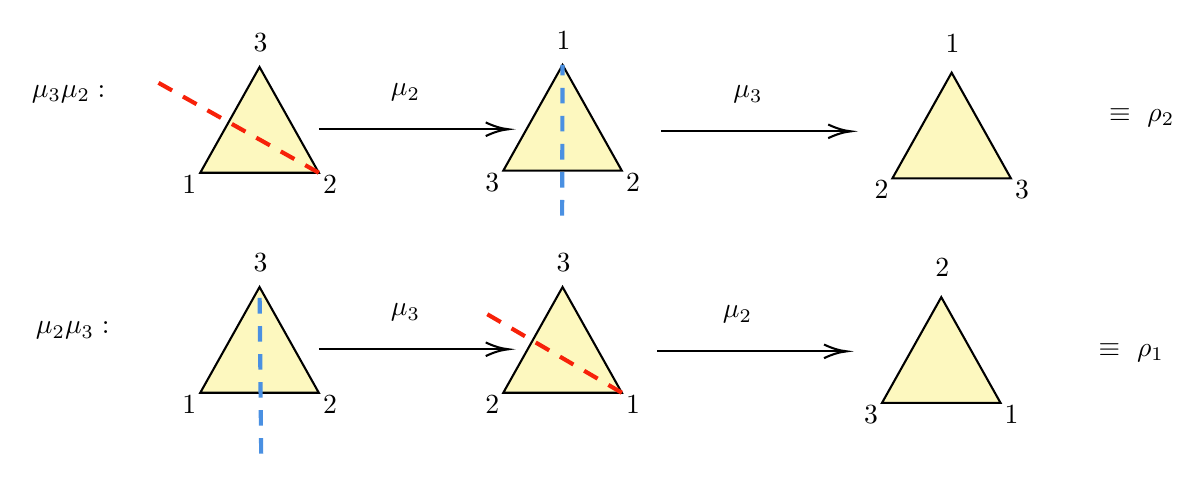
\begin{tikzpicture}[x=0.75pt,y=0.75pt,yscale=-1,xscale=1]
%uncomment if require: \path (0,222); %set diagram left start at 0, and has height of 222

%Straight Lines [id:da07468523150361062] 
\draw    (365.75,63.24) -- (455.12,63.24) ;
\draw [shift={(457.12,63.24)}, rotate = 180] [color={rgb, 255:red, 0; green, 0; blue, 0 }  ][line width=0.75]    (10.93,-3.29) .. controls (6.95,-1.4) and (3.31,-0.3) .. (0,0) .. controls (3.31,0.3) and (6.95,1.4) .. (10.93,3.29)   ;
%Straight Lines [id:da7303972534757194] 
\draw    (363.75,169.24) -- (453.12,169.24) ;
\draw [shift={(455.12,169.24)}, rotate = 180] [color={rgb, 255:red, 0; green, 0; blue, 0 }  ][line width=0.75]    (10.93,-3.29) .. controls (6.95,-1.4) and (3.31,-0.3) .. (0,0) .. controls (3.31,0.3) and (6.95,1.4) .. (10.93,3.29)   ;
%Shape: Triangle [id:dp3013799303944148] 
\draw  [fill={rgb, 255:red, 250; green, 238; blue, 106 }  ,fill opacity=0.43 ] (505.67,34.97) -- (534.22,85.91) -- (477.11,85.91) -- cycle ;
%Shape: Triangle [id:dp8366420155668731] 
\draw  [fill={rgb, 255:red, 250; green, 238; blue, 106 }  ,fill opacity=0.43 ] (500.67,143.13) -- (529.22,194.08) -- (472.11,194.08) -- cycle ;
%Shape: Triangle [id:dp08911820327135123] 
\draw  [fill={rgb, 255:red, 250; green, 238; blue, 106 }  ,fill opacity=0.43 ] (318.21,31.26) -- (346.76,82.2) -- (289.65,82.2) -- cycle ;

%Shape: Triangle [id:dp6959388954166472] 
\draw  [fill={rgb, 255:red, 250; green, 238; blue, 106 }  ,fill opacity=0.43 ] (172.21,32.26) -- (200.76,83.2) -- (143.65,83.2) -- cycle ;

%Straight Lines [id:da28918778113624566] 
\draw [color={rgb, 255:red, 247; green, 33; blue, 9 }  ,draw opacity=1 ][line width=1.5]  [dash pattern={on 5.63pt off 4.5pt}]  (200.76,83.2) -- (123,39.58) ;
%Straight Lines [id:da8925263126633919] 
\draw    (200.75,62.24) -- (290.12,62.24) ;
\draw [shift={(292.12,62.24)}, rotate = 180] [color={rgb, 255:red, 0; green, 0; blue, 0 }  ][line width=0.75]    (10.93,-3.29) .. controls (6.95,-1.4) and (3.31,-0.3) .. (0,0) .. controls (3.31,0.3) and (6.95,1.4) .. (10.93,3.29)   ;
%Shape: Triangle [id:dp5381554452767219] 
\draw  [fill={rgb, 255:red, 250; green, 238; blue, 106 }  ,fill opacity=0.43 ] (318.21,138.26) -- (346.76,189.2) -- (289.65,189.2) -- cycle ;

%Shape: Triangle [id:dp9555744124634001] 
\draw  [fill={rgb, 255:red, 250; green, 238; blue, 106 }  ,fill opacity=0.43 ] (172.21,138.26) -- (200.76,189.2) -- (143.65,189.2) -- cycle ;

%Straight Lines [id:da6550087809178868] 
\draw    (200.75,168.24) -- (290.12,168.24) ;
\draw [shift={(292.12,168.24)}, rotate = 180] [color={rgb, 255:red, 0; green, 0; blue, 0 }  ][line width=0.75]    (10.93,-3.29) .. controls (6.95,-1.4) and (3.31,-0.3) .. (0,0) .. controls (3.31,0.3) and (6.95,1.4) .. (10.93,3.29)   ;
%Straight Lines [id:da7497507878697739] 
\draw [color={rgb, 255:red, 74; green, 144; blue, 226 }  ,draw opacity=1 ][line width=1.5]  [dash pattern={on 5.63pt off 4.5pt}]  (173,218.57) -- (172.21,138.26) ;
%Straight Lines [id:da38955785017328814] 
\draw [color={rgb, 255:red, 247; green, 33; blue, 9 }  ,draw opacity=1 ][line width=1.5]  [dash pattern={on 5.63pt off 4.5pt}]  (346.76,189.2) -- (280,150.23) ;
%Straight Lines [id:da7214149866229602] 
\draw [color={rgb, 255:red, 74; green, 144; blue, 226 }  ,draw opacity=1 ][line width=1.5]  [dash pattern={on 5.63pt off 4.5pt}]  (318,103.83) -- (318.21,31.26) ;

% Text Node
\draw (63,153.63) node [anchor=north west][inner sep=0.75pt]    {$\mu _{2} \mu _{3} :$};
% Text Node
\draw (61,39.63) node [anchor=north west][inner sep=0.75pt]    {$\mu _{3} \mu _{2} :$};
% Text Node
\draw (399,39.91) node [anchor=north west][inner sep=0.75pt]    {$\mu _{3}$};
% Text Node
\draw (394,145.91) node [anchor=north west][inner sep=0.75pt]    {$\mu _{2}$};
% Text Node
\draw (467.03,85.7) node [anchor=north west][inner sep=0.75pt]    {$2$};
% Text Node
\draw (534.75,85.7) node [anchor=north west][inner sep=0.75pt]    {$3$};
% Text Node
\draw (501.3,14.98) node [anchor=north west][inner sep=0.75pt]    {$1$};
% Text Node
\draw (462.03,193.87) node [anchor=north west][inner sep=0.75pt]    {$3$};
% Text Node
\draw (529.75,193.87) node [anchor=north west][inner sep=0.75pt]    {$1$};
% Text Node
\draw (496.3,123.15) node [anchor=north west][inner sep=0.75pt]    {$2$};
% Text Node
\draw (234,38.91) node [anchor=north west][inner sep=0.75pt]    {$\mu _{2}$};
% Text Node
\draw (167.84,14.8) node [anchor=north west][inner sep=0.75pt]    {$3$};
% Text Node
\draw (201.29,83) node [anchor=north west][inner sep=0.75pt]    {$2$};
% Text Node
\draw (133.57,83) node [anchor=north west][inner sep=0.75pt]    {$1$};
% Text Node
\draw (313.84,13.8) node [anchor=north west][inner sep=0.75pt]    {$1$};
% Text Node
\draw (347.29,82) node [anchor=north west][inner sep=0.75pt]    {$2$};
% Text Node
\draw (279.57,82) node [anchor=north west][inner sep=0.75pt]    {$3$};
% Text Node
\draw (234,144.91) node [anchor=north west][inner sep=0.75pt]    {$\mu _{3}$};
% Text Node
\draw (167.84,120.8) node [anchor=north west][inner sep=0.75pt]    {$3$};
% Text Node
\draw (201.29,189) node [anchor=north west][inner sep=0.75pt]    {$2$};
% Text Node
\draw (133.57,189) node [anchor=north west][inner sep=0.75pt]    {$1$};
% Text Node
\draw (313.84,120.8) node [anchor=north west][inner sep=0.75pt]    {$3$};
% Text Node
\draw (347.29,189) node [anchor=north west][inner sep=0.75pt]    {$1$};
% Text Node
\draw (279.57,189) node [anchor=north west][inner sep=0.75pt]    {$2$};
% Text Node
\draw (575,163.97) node [anchor=north west][inner sep=0.75pt]    {$\equiv \ \rho _{1}$};
% Text Node
\draw (580,50.97) node [anchor=north west][inner sep=0.75pt]    {$\equiv \ \rho _{2}$};


\end{tikzpicture}
